\chapter{AMSR data}
\label{chap:amsr}

\section{AMSR introduction}
\label{sec:amsr_intro}

\section{AMSR data statistical analysis}
\label{sec:amsr_statstical}
The AMSR measurement coefficient matrix is given in the Tab.\ref{tab:covariance_AMSR}. Fig.\ref{fig:pdf33} and Fig.\ref{fig:pdf58} shows the estimated probability density basing on the AMSR data measured during $1^{st},1,2005-14^{th},1,2005$ period of location 33 and location 58. The ideal normal distribution with the variance extracted from Tab.\ref{tab:covariance_AMSR} and the average Tb as the mean is plotted together for comparison.   
\begin{table}[h]
   \begin{tabular}{|c|cccccccccc|}
\hline
Channel   & 6GV&6GH&11GV&11GH&19GV&19GH&23GV&23GH&37GV&37GH\\
\hline
6GV& 0.09&      0&      0&      0&      0&       0&      0&      0&      0&      0\\  
6GH&    0&0.1089&      0&      0&      0&       0&      0&      0&      0&      0\\  
11GV&    0&     0& 0.2209&      0&      0&       0&      0&      0&      0&      0\\
11GH&    0&     0&      0& 0.2916&      0&       0&      0&      0&      0&      0\\
19GV&    0&     0&      0&      0& 0.2304&       0&      0&      0&      0&      0\\
19GH&    0&     0&      0&      0&      0& 0.2116&      0&      0&      0&      0\\
23GV&    0&     0&      0&      0&      0&      0& 0.2025&      0&      0&      0\\
23GH&    0&     0&      0&      0&      0&      0&      0& 0.1936&      0&      0\\
37GV&    0&     0&      0&      0&      0&      0&      0&      0& 0.2025&      0\\ 
37GH&    0&     0&      0&      0&      0&      0&      0&      0&       0&     0.16\\
\hlilne
  \end{tabular}
 \caption{Covariance matrix of AMSR measurements}
 \label{tab:covariance_AMSR}
\end{table}

\begin{figure}[hbp]
  \centering
   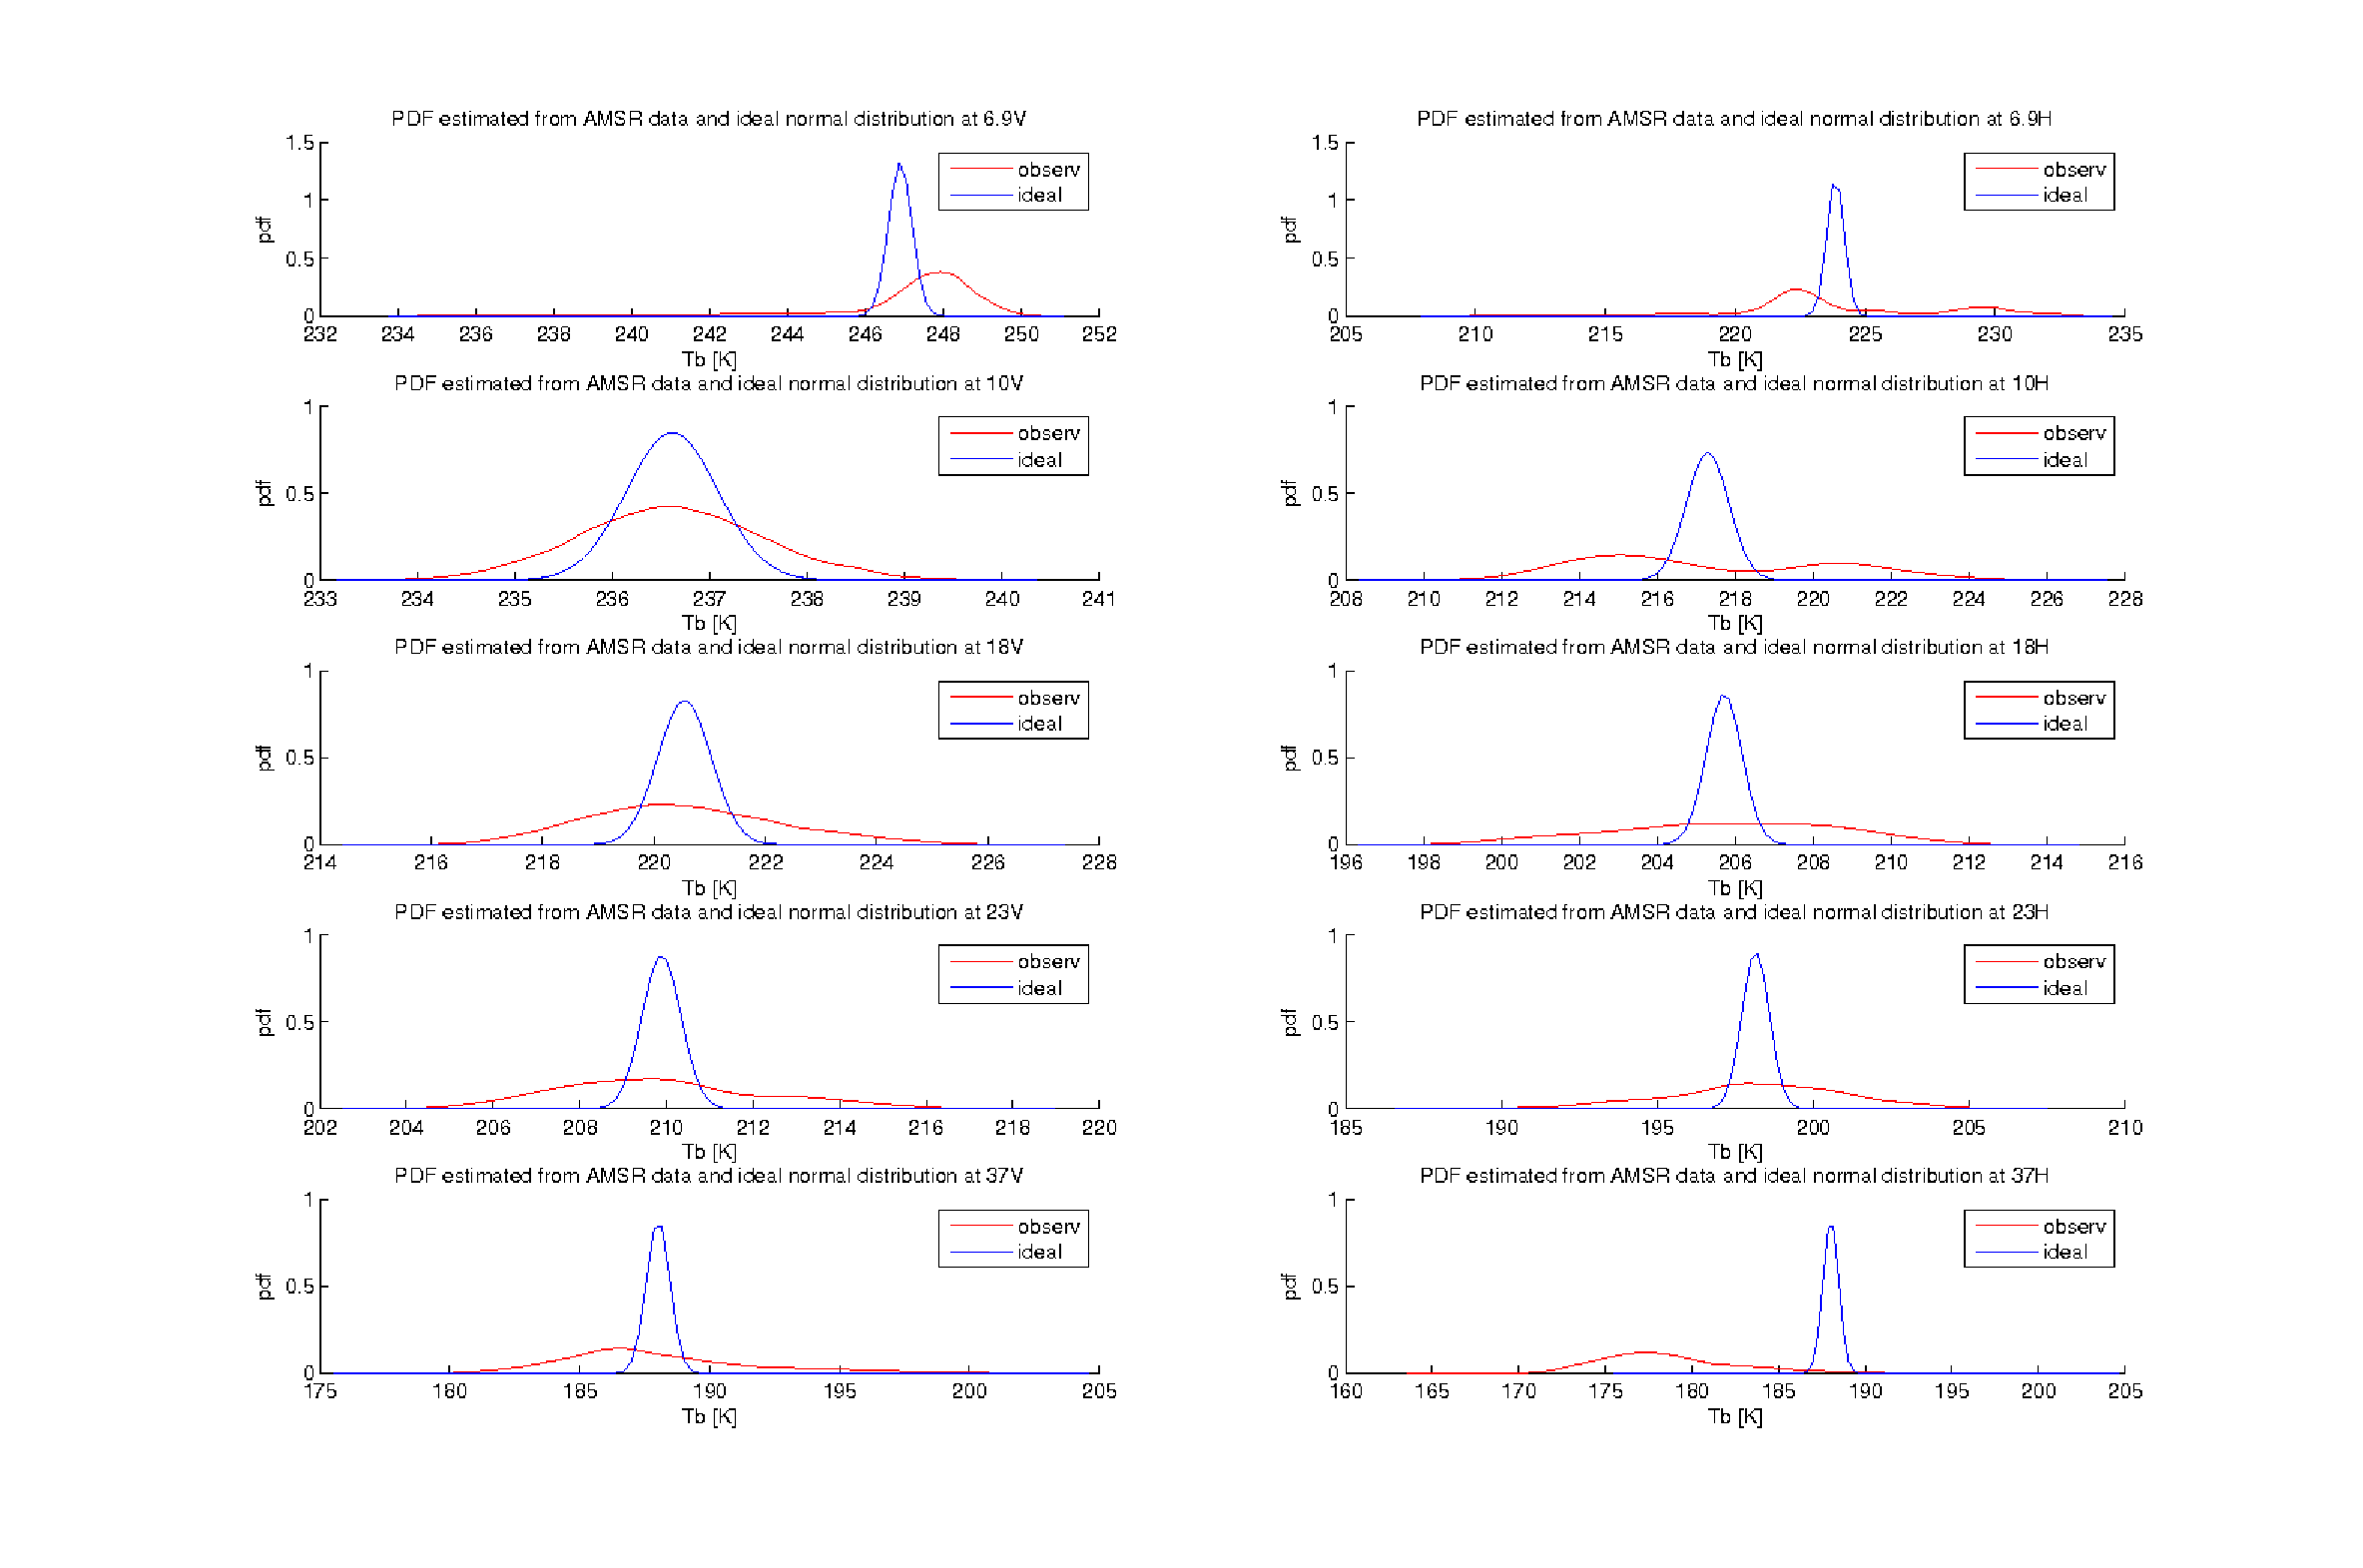
\includegraphics[width=0.45]{pdf33.eps} 
  \caption{Estimated pdf of AMSR data at loc.58.}
  \label{fig:pdf33}
\end{figure}

\clearpage

\begin{figure}[hbp]
  \centering
   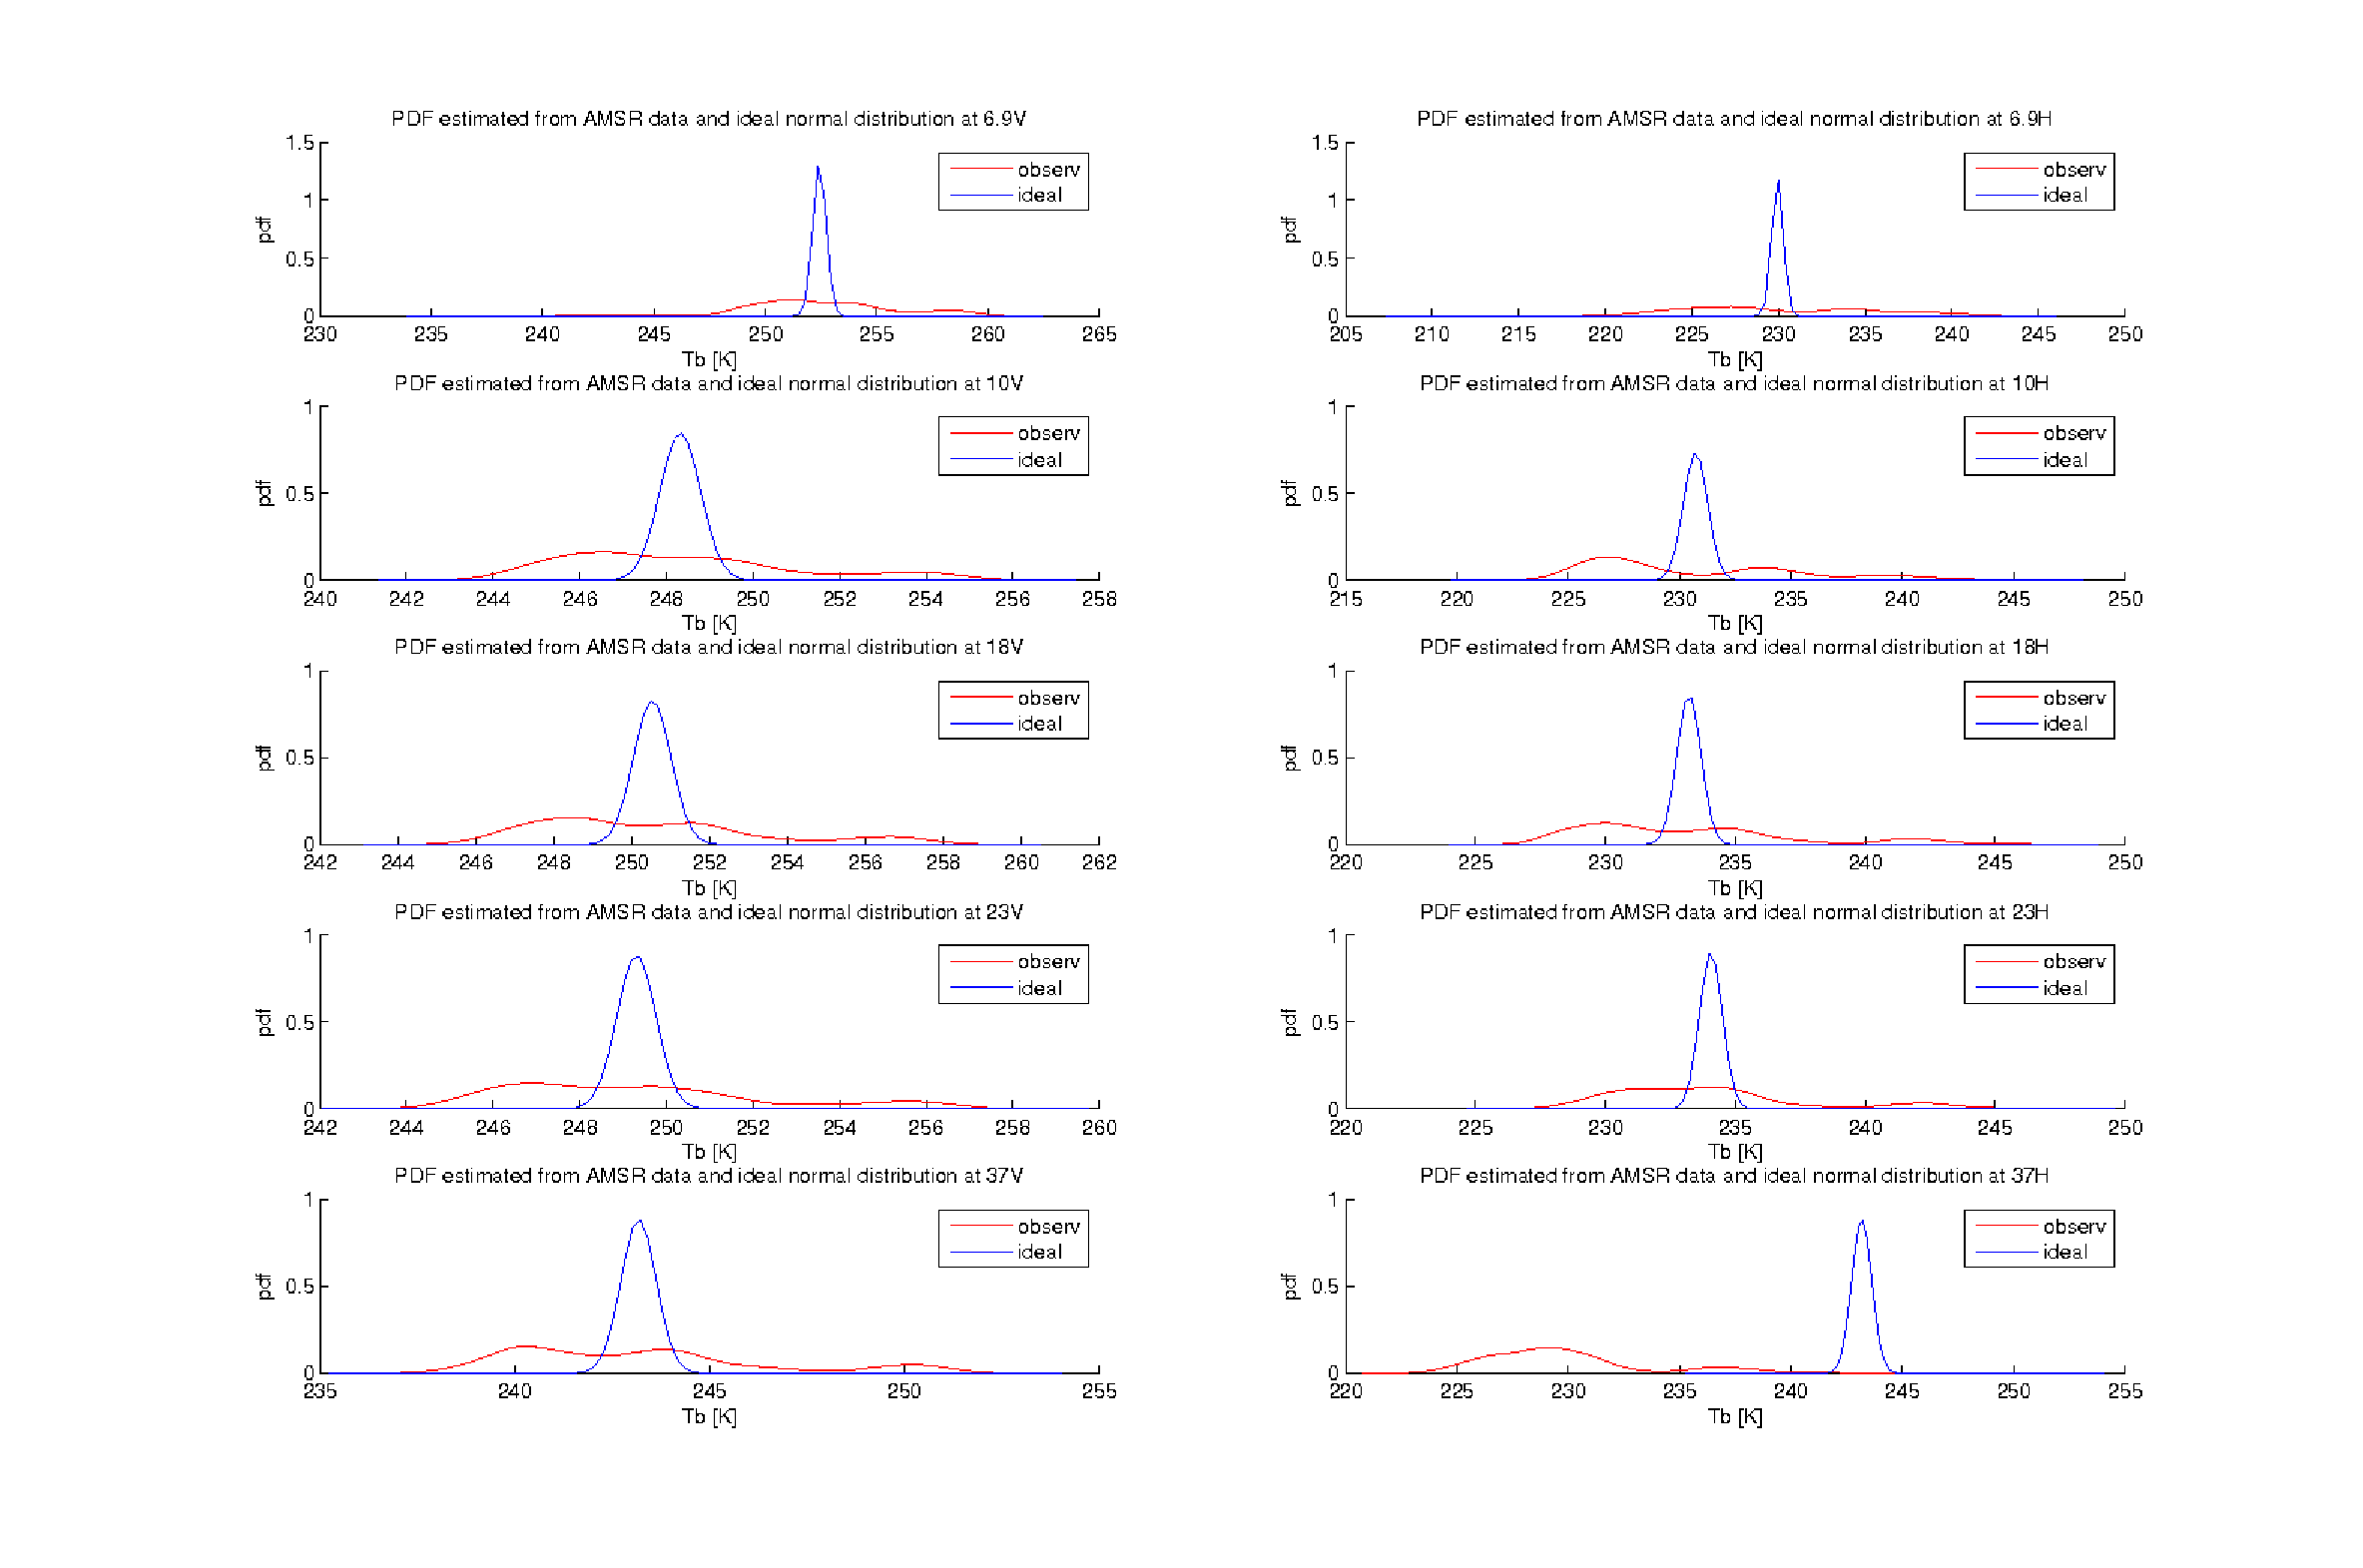
\includegraphics[width=0.45]{pdf58.eps} 
  \caption{Estimated pdf of AMSR data at loc.58}
  \label{fig:pdf58}
\end{figure}
\clearpage
